\documentclass[compress,mathserif]{beamer}
\usepackage[latin2]{inputenc}
%\usepackage[absolute]{textpos}
%\documentclass[handout,compress,mathserif]{beamer}
%\setbeameroption{show notes}

% This file is a solution template for:

% - Talk at a conference/colloquium.
% - Talk length is about 20min.
% - Style is ornate.



% Copyright 2004 by Till Tantau <tantau@users.sourceforge.net>.
%
% In principle, this file can be redistributed and/or modified under
% the terms of the GNU Public License, version 2.
%
% However, this file is supposed to be a template to be modified
% for your own needs. For this reason, if you use this file as a
% template and not specifically distribute it as part of a another
% package/program, I grant the extra permission to freely copy and
% modify this file as you see fit and even to delete this copyright
% notice.


\mode<presentation>
{
  %\usetheme{pittsburgh}
  % or ...

  \setbeamercovered{invisible}
  \useoutertheme[subsection=false]{miniframes}
  % or whatever (possibly just delete it)
}


\usepackage[USenglish]{babel}
%\usepackage[latin1]{inputenc}
\usepackage[T1]{fontenc}
%\usepackage{mathpazo}
\usepackage{ifthen,array}

\pretolerance5000 \hyphenpenalty9999
%\setlength{\TPHorizModule}{0.5cm} \setlength{\TPVertModule}{0.5cm}
%\textblockorigin{20mm}{20mm} % start everything near the top-left corner

\newcounter{ora}
\newcounter{perc}
\newcounter{kezdoora}
\newcounter{kezdoperc}
\newcounter{percek}
\setcounter{percek}{0}
\setcounter{kezdoora}{0} % for 1.35pm as the starting time

\providecommand{\leadingzero}[1]{\ifthenelse{\value{#1}<10}{0\arabic{#1}}{\arabic{#1}}}
\providecommand{\oradisplay}[1]{\ifthenelse{\value{#1}<60}{\arabic{kezdoora}:\leadingzero{#1}}{\setcounter{perc}{\value{#1}}\addtocounter{perc}{-60}\setcounter{ora}{\value{kezdoora}}\addtocounter{ora}{1}\arabic{ora}:\leadingzero{perc}}}

\providecommand{\notes}[1]{{\tiny\textbf{Note:} #1}}
%%%%%%%%%%%%%%%%%%%%%%%%%%%%%%%%%%%%%%%%%%%%%%%%
%% Hasznos matek makrok
%%%%%%%%%%%%%%%%%%%%%%%%%%%%%%%%%%%%%%%%%%%%%%%%

\newcommand{\QED}{{}\hfill$\Box$}
\newcommand{\intl}[4]{\int_{#1}^{#2} \! {#3} \, \mathrm d{#4}}
\newcommand{\period}{\text{.}} % Ez azert kell, mert a matek . mashogy nez ki, mint a szovege.
\newcommand{\comma}{\text{,}}  % Ez azert kell, mert a matek , mashogy nez ki, mint a szovege.
\newcommand{\dist}{\,\mathop{\operatorname{\sim\,}}\limits}
\newcommand{\D}{\,\mathop{\operatorname{d}}\!}
%\newcommand{\E}{\mathop{\operatorname{E}}\nolimits}
\newcommand{\Lag}{\mathop{\operatorname{L}}}
\newcommand{\plim}{\mathop{\operatorname{plim}}\limits_{T\to\infty}\,}
\newcommand{\CES}[3]{\mathop{\operatorname{CES}}\left(\left\{#1\right\},\left\{#2\right\},#3\right)}
\newcommand{\cestwo}[5]{\left[#1^\frac1{#5}\,#2^\frac{#5-1}{#5}+#3^\frac1{#5}\,#4^\frac{#5-1}{#5}\right]^\frac{#5}{#5-1}}
\newcommand{\cesmore}[4]{\left[\sum_{#3}#1_{#3}^\frac1{#4}\,{#2}_{#3}^\frac{#4-1}{#4}\right]^\frac{#4}{#4-1}}
\newcommand{\cesPtwo}[5]{\left[#1\,#2^{1-#5}+#3\,#4^{1-#5}\right]^\frac{1}{1-#5}}
\newcommand{\cesPmore}[4]{\left[\sum_{#3}#1_{#3}\,#2_{#3}^{1-#4}\right]^\frac{1}{1-#4}}
\newcommand{\diff}[2]{\frac{\D #1}{\D #2}}
\newcommand{\pdiff}[2]{\frac{\partial #1}{\partial #2}}
\newcommand{\convex}[2]{\lambda #1 + (1-\lambda)#2}
\newcommand{\ABS}[1]{\left| #1 \right|}
\newcommand{\suchthat}{:\hskip1em}
\newcommand{\dispfrac}[2]{\frac{\displaystyle #1}{\displaystyle #2}} % Emeletes tortekhez hasznos.

\newcommand{\diag}{\mathop{\mathrm{diag\mathstrut}}}
\newcommand{\tr}{\mathop{\mathrm{tr\mathstrut}}}
\newcommand{\E}{\mathop{\mathrm{E\mathstrut}}}
\newcommand{\Var}{\mathop{\mathrm{Var\mathstrut}}\nolimits}
\newcommand{\Cov}{\mathop{\mathrm{Cov\mathstrut}}}
\newcommand{\sgn}{\mathop{\operatorname{sgn\mathstrut}}}

\newcommand{\covmat}{\mathbf\Sigma}
\newcommand{\ones}{\mathbf 1}
\newcommand{\zeros}{\mathbf 0}
\newcommand{\BAR}[1]{\overline{#1}}


\newlength{\tempsep}

\newenvironment{subeqs}{\setlength{\tempsep}{\arraycolsep}
\setlength{\arraycolsep}{0.13889em} % Ez azert kell, hogy ne hagyjon tul sok helyet az = korul.
\begin{subequations}\begin{eqnarray}}
{\end{eqnarray}\end{subequations}
\setlength{\arraycolsep}{\tempsep}}

\newenvironment{tapad}{\setlength{\tempsep}{\arraycolsep}
\setlength{\arraycolsep}{0.13889em}} % Ez azert kell, hogy ne hagyjon tul sok helyet az = korul.
{\setlength{\arraycolsep}{\tempsep}}

\newenvironment{eqnarr}{\setlength{\tempsep}{\arraycolsep}
\setlength{\arraycolsep}{0.13889em} % Ez azert kell, hogy ne hagyjon tul sok helyet az = korul.
\begin{eqnarray}}
{\end{eqnarray} \setlength{\arraycolsep}{\tempsep}}

\newenvironment{eqnarr*}{\setlength{\tempsep}{\arraycolsep}
\setlength{\arraycolsep}{0.13889em} % Ez azert kell, hogy ne hagyjon tul sok helyet az = korul.
\begin{eqnarray*}}
{\end{eqnarray*} \setlength{\arraycolsep}{\tempsep}}


%\usepackage[active]{srcltx} % SRC Specials: DVI [Inverse] Search
% Fuzz --- -------------------------------------------------------
\hfuzz5pt % Don't bother to report over-full boxes < 5pt
\vfuzz5pt % Don't bother to report over-full boxes < 5pt
% THEOREMS -------------------------------------------------------
% MATH -----------------------------------------------------------
\newcommand{\norm}[1]{\left\Vert#1\right\Vert}
\newcommand{\abs}[1]{\left\vert#1\right\vert}
\newcommand{\set}[1]{\left\{#1\right\}}
\newcommand{\Real}{\mathbb R}
\newcommand{\eps}{\varepsilon}
\newcommand{\To}{\longrightarrow}
\newcommand{\BX}{\mathbf{B}(X)}
\newcommand{\A}{\mathcal{A}}

%\renewcommand{\rmdefault}{pmnr}
%\renewcommand{\sfdefault}{iwona}



\newcommand{\directory}{figures}
\newcommand*{\newtitle}{\egroup\begin{frame}\frametitle}

\newcommand{\fullpagefigure}[2]{\begin{frame}\frametitle{\hyperlink{#1back}{#2}}\hypertarget{#1}{{\begin{center}\includegraphics[height=0.9\textheight]{\directory/#1}\end{center}}}\end{frame}}
\newcommand{\widefigure}[2]{\begin{frame}\frametitle{\hyperlink{#1back}{#2}}\hypertarget{#1}{{\begin{center}\label{#1}\includegraphics[width=\linewidth]{\directory/#1}\end{center}}}\end{frame}}
\newcommand{\longfigure}[2]{\begin{frame}\frametitle{\hyperlink{#1back}{#2}}\hypertarget{#1}{{\begin{center}\includegraphics[height=0.8\textheight]{\directory/#1}\end{center}}}\end{frame}}
%\newcommand{\fullpagefigure}[2]{\begin{frame}\frametitle{\hyperlink{#1back}{#2}}\hypertarget{#1}{{\begin{centering}$#1$\end{centering}}}\end{frame}}
\newcommand{\answer}[1]{\begin{itemize}\item #1\end{itemize}}


\newcommand{\jumpto}[2]{\hypertarget{#1back}{\hyperlink{#1}{#2}}}
\newcommand{\backto}[2]{\hypertarget{#1}{\hyperlink{#1back}{#2}}}

\renewcommand{\time}[1]{\addtocounter{percek}{#1}}

\title[Balassa--Samuelson]% (optional, use only with long paper titles)
{A Spatial Explanation for the\\ Balassa--Samuelson Effect}


\author[Karadi and Koren] % (optional, use only with lots of authors)
{Peter Karadi (NYU)\\
Miklos Koren (Central European University and CEPR)}
% - Give the names in the same order as the appear in the paper.
% - Use the \inst{?} command only if the authors have different
%   affiliation.


\date % (optional, should be abbreviation of conference name)
{}
% - Either use conference name or its abbreviation.
% - Not really informative to the audience, more for people (including
%   yourself) who are reading the slides online

%\subject{Theoretical Computer Science}
% This is only inserted into the PDF information catalog. Can be left
% out.



% If you have a file called "university-logo-filename.xxx", where xxx
% is a graphic format that can be processed by latex or pdflatex,
% resp., then you can add a logo as follows:

%\pgfdeclareimage[height=0.5cm]{university-logo}{frblogo}
%\logo{\pgfuseimage{university-logo}}



% Delete this, if you do not want the table of contents to pop up at
% the beginning of each subsection:
\AtBeginSection[]
{
  \begin{frame}[plain]
    \frametitle{\color{red}\insertsection}
    \addtocounter{framenumber}{-1}
    %\tableofcontents[currentsection,currentsubsection]
  \end{frame}
}


% If you wish to uncover everything in a step-wise fashion, uncomment
% the following command:

%\beamerdefaultoverlayspecification{<+->}

%\setbeamertemplate{navigation symbols}{}
%\setbeamertemplate{footline}{{}\hfill\insertframenumber--\oradisplay{percek}}

\begin{document}

\begin{frame}[plain]
  \titlepage
    \addtocounter{framenumber}{-1}
\end{frame}


\section{Introduction}

\subsection{Motivation}
\begin{frame}\frametitle{The Balassa--Samuelson effect}

\begin{itemize}
    \item<1-> Rich countries are more expensive than poor ones.
    \item<1-> In the Penn World Table,
    \[
    \ln P = 0.25\ln Y + e.
    \]
    %% The reason I put in numbers here is that I want to be able to do back of the env calcs.
    \item<2-> This is mostly due to differences in non-tradable prices, as tradable prices vary little across countries.
        \hyperlink{shampoo}{\beamerbutton{Shampoo}}
    \item<3-> Over time, as a country grows, its non-tradables become relatively more expensive.         \hyperlink{US_VA_prices}{\beamerbutton{US prices}}

\end{itemize}
\end{frame}

\time{2}

\subsection{}

\begin{frame}\frametitle{What we do}

\begin{itemize}
    \item We propose a simple spatial model in which relative price changes arise endogenously from the location choice of industries.
    \item Industries share the exact same technology, they only differ in \emph{tradability}.
\end{itemize}

%% emphasize that this conforms to our notion of tradability
\end{frame}

\begin{frame}\frametitle{Basic idea}
\begin{itemize}
    \item Tradable sectors locate to where land is cheap.
    \item Non-tradable sectors have to locate near consumers in big cities.
%    \item They compete with housing for scarce urban land.
    \item Urban land becomes more and more scarce with development.
    \item Raising the relative price of non-tradables.
\end{itemize}
\end{frame}
\time{2}

\begin{frame}\frametitle{Alternative explanations}

\begin{itemize}
    \item<1-> Balassa--Samuelson: Productivity growth in non-tradables is slower than in tradables. \hyperlink{PPF-balassa}{\beamerbutton{Balassa}}
    \item<2-> Bhagwati--Kravis--Lipsey: Non-tradables are more intensive users of the non-reproducible factor (labor).
    \item<2-> This raises their price with capital accumulation.\hyperlink{PPF-bhagwati}{\beamerbutton{Bhagwati}}
\end{itemize}
\end{frame}

\begin{frame}\frametitle{Issues with the alternative explanations}

\begin{itemize}
    \item<1-> Where do technology differences come from?
    \item<2-> Factor intensity differences seem to be small. \hyperlink{Valentinyi}{\beamerbutton{Income shares}}
    \item<3-> Why does Balassa--Samuelson work in some cases and not in others? \hyperlink{sc_penn}{\beamerbutton{Urban}} \hyperlink{chicken}{\beamerbutton{Chicken}}
\end{itemize}
\end{frame}

%% however, both of these technology assumptions are rather ad hoc. they will never be able to explain variations in the BS effect. as we will see, there is substantial variation both across countries and over time (in particular, BS is relatively recent). our model will be able to speak to both.

%\section{What we do}

%% talk about outline: 1. land matters. 2. simple model. 3. some supportive evidence


\section{Location matters}
\subsection{}

%% do we need this for the madrid audience?
\widefigure{clark-landrents}{Why has land disappeared from macro?\\ (Clark, 2007)}

\begin{frame}\frametitle{Land is scarce}
\begin{itemize}
    \item Population density of the Earth is 42$/\text{km}^2$, so land is abundant.
    \pause
    \item However, the average person lives in an area with a population density of 7,300$/\text{km}^2$ (LandScan 2005),
    so \emph{land close to consumers} is scarce.
\end{itemize}
\end{frame}
\time 2

%% as a comparison, NYC is 10,000
%% Madrid is 5,300


\section{Firms}
\subsection{}

\subsection{Basic structure}
\begin{frame}\frametitle{Basic structure}
\begin{itemize}
    \item There are two sectors, manufacturing ($m$) and services ($s$).
    \item We study how the relative prices of these industries depend on their choice of location...
    \item ...and how location varies with development.
\end{itemize}
\end{frame}

\begin{frame}\frametitle{Spatial structure}
\begin{itemize}
    \item We use the monocentric city model.
    \item All market exchange takes place in a central business district (CBD).
    \item CBD is a point on the real line.
    \item Manufacturing and service establishments can choose their location freely on the real line.
    \item Location is indexed by distance to the CBD, $z$.
\end{itemize}
\end{frame}

\time{2}

\begin{frame}\frametitle{Technology}
\begin{itemize}
    \item Land is the only factor of production.
    \item Production functions:
\begin{align*}
m&=A_ml_m\\
s&=A_sl_s
\end{align*}
\end{itemize}
\end{frame}

\time{1}

%% we may want to introduce exponential right away
\begin{frame}\frametitle{Transport costs}
\begin{itemize}
    \item Goods are shipped to the CBD.
    \item Both manufacturing and services have iceberg transport cost.
    \item One good $i$ shipped from location $z$ melts to \hyperlink{Dz-exp}{\beamerbutton{iceberg}}
    \[
    {e}^{-\tau_iz}.
    \]
    \item Services are less tradable:
    \[
    \tau_s>\tau_m.
    \]
\end{itemize}
\end{frame}
\time{2}

%%% compress this into one bullet list
\subsection{Equilibrium}

\begin{frame}\frametitle{Profit maximization}
\begin{itemize}
    \item Land rent at location $z$: $r(z)$.
    \item Profits for industry $i$ at location $z$:
    \[
    {e}^{-\tau_i z} p_i A_i l_i(z) - r(z)l_i(z).
    \]
    \item Optimum requires
    \[
    {e}^{-\tau_i z} p_i A_i \le r(z),
    \]
    with equality if industry $i$ produces at location $z$.
\end{itemize}
\end{frame}
\time{1}

\begin{frame}\frametitle{The bid rent curve$\cdot$}
\begin{itemize}
    \item Define a bid rent curve:
    \[
    R_i(z) = p_iA_i{e}^{-\tau_i z}.
    \]
    \item Profit maximization requires
    \[
    r(z)\ge R_i(z)
    \]
    \item Industry $i$ produces at location $z$ only if equal \hyperlink{bid-rent-2-exp}{\beamerbutton{bid rent}}
    \item Rent $r(z)$ is the upper envelope of the bid rent curves.
\end{itemize}
\end{frame}

%% production possibilities frontier here
\begin{frame}\frametitle{Optimal location choice}
\begin{itemize}
\item Services are produced between $0$ and $\Bar z$:
\[
s = \int_0^{\Bar z}A_se^{-\tau_s z}dz.
\]
\item Manufacturing takes place between $\Bar z$ and $\infty$.
\[
m = \int_{\Bar z}^\infty A_me^{-\tau_m z}dz.
\]
\item Production possibilities frontier \hyperlink{PPF-location}{\beamerbutton{PPF}}:
\[
s = \frac{A_s}{\tau_s}\left[1-\left(\frac{m}{A_m/\tau_m}\right)^{\tau_s/\tau_m}\right]
\]
%\item Marginal rate of transformation:
%\[
%MRT = %\frac{A_m}{A_s}\left(\frac{m}{A_m/\tau_m}\right)^{-(\tau_s-\tau_m)/\tau_m}
%\]
\end{itemize}
\end{frame}

\begin{frame}\frametitle{Balassa--Samuelson with location-specific land}
\begin{itemize}
\item Trade costs make land location specific: ``urban'' land is different from ``rural'' land.
\item Services are more intensive users of ``urban'' land.
\item With only trade cost differences across sectors, service price increases if and only if ``urban'' land becomes \emph{scarce} relative to ``rural'' land.
\end{itemize}
\end{frame}
%% 2-fctor wording may be misleading

%% next step: why does manufacturing shrink with development?
\subsection{Manufacturing and development}

\begin{frame}\frametitle{Manufacturing and development}
\label{development}
Urban land may become relatively scarce for a number of reasons.
\begin{enumerate}
\item<1-> Manufacturing shipping costs decline disproportionately. \hyperlink{transport}{\beamerbutton{Transport cost}}
\item<1-> Structural change shifts resources towards services. \hyperlink{Structchange}{\beamerbutton{Structural change}}
\item<2-> Development increases the demand for residential land. \hyperlink{housing}{\beamerbutton{Housing}}
\end{enumerate}
\end{frame}
\time 1

\section{Consumers}
\subsection{}

\begin{frame}\frametitle{Tastes}
\begin{itemize}
    \item Consumers have homothetic utility over $m$, $s$ and $h$.
    \item With indirect utility function
    \[
    u(I,p_m,p_s,p_h) = \frac{I}{P(p_m,p_s,p_h)}.
    \]
    \item Assume nested structure
    \[
    P[\Phi(p_m,p_s),p_h].
    \]
\end{itemize}
\end{frame}

\begin{frame}\frametitle{Commuting costs}
\begin{itemize}
    \item People go to the CBD to shop.
    \item Commuting costs a $1-{e}^{-\tau_h z}$ fraction of the consumption bundle.
    \item So that indirect utility is
    \[
    u(I,p_m,p_s,p_h) = \frac{{e}^{-\tau_h z}I}{P[\Phi(p_m,p_s),p_h]}.
    \]
    \item Commuting is the costliest of all,
    \[
    \tau_h>\tau_s>\tau_m.
    \]
\end{itemize}
\end{frame}
\time{1}

%% skip this
\begin{frame}\frametitle{The bid rent curve of households$\cdot$}
\begin{itemize}
    \item Housing at $z$ costs $r(z)/A_h$.
    \item Other two prices do not depend on residence.
    \item To achieve utility $u$ at location $z$,
    \[
    u = \frac{{e}^{-\tau_h z} I}{P[\Phi(p_m,p_s),r(z)/A_h]}.
    \]
    \item Bid rent function
    \[
    R_h(z) = A_h\Phi(p_m,p_s)P_2^{-1}\left[\frac{{e}^{-\tau_h z} I}{u\Phi(p_m,p_s)}\right].
    \]
    \item For example, with Cobb--Douglas utility,
\[
R_h(z) = A_h\left[\frac{{e}^{-\tau_h z} I}{up_m^{\alpha}p_s^{\beta}}\right]^{1/\gamma}.
\]
\end{itemize}
\end{frame}
%\time{2}

\begin{frame}\frametitle{Equilibrium spatial structure}
There exists a unique equilibrium.
\begin{itemize}
    \item Residents live closest to CBD, $\in[0,\underline{z}]$.
    \item With a (weakly) declining population density.
    \item Followed by an interval of service establishments, $\in(\underline{z},\overline{z}]$.
    \item Followed by an interval of manufacturing plants, $\in(\overline{z},\infty)$.
%    \item The boundaries $z_1$ and $z_2$ determine the supply of housing
\end{itemize}
\end{frame}

\begin{frame}\frametitle{Finding the equilibrium $\underline{z}$ and $\overline{z}$}
\begin{itemize}
    \item Cutoffs pin down supply:
    \begin{align*}
    s &= A_s\int_{\underline{z}}^{\overline{z}}{e}^{-\tau_s z} dz, \\
    m &= A_m\int_{\overline{z}}^{\infty}{e}^{-\tau_m z} dz .
    \end{align*}
    \item Arbitrage at the manufacturing--service boundary $\overline{z}$ pins down relative prices,
    \[
    p_mA_m{e}^{-\tau_m \overline{z}} = p_sA_s{e}^{-\tau_s \overline{z}},
    \]
    which determines demand.
    \item Find $\underline{z}$ and $\overline{z}$ such that markets clear.
\end{itemize}
\end{frame}
\time 2

%\subsection{Housing}

\begin{frame}\frametitle{Productivity growth}
\begin{itemize}
\item We conduct the following comparative statics.
\item Increase $A_m$ and $A_s$ proportionally (so that productivity growth is neutral).
\item What happens to industry location ($\underline{z}$, $\overline{z}$) and relative prices?
\end{itemize}
\end{frame}
\time 1

\begin{frame}\frametitle{Propositions}

\begin{block}{Balassa--Samuelson and the sprawl}
Service prices increase with development if and only if residential land increases with development.
\end{block}
\pause

\begin{block}{Balanced growth}
Productivity growth does not change the relative price of services if
    \begin{enumerate}
      \item housing productivity grows at the same rate,
      \item \emph{or} demand for housing is Cobb--Douglas.
    \end{enumerate}
\end{block}
\end{frame}
\time 3
%% explain C-D

%% explain sprawl

%\subsection{Comparative statics}

\begin{frame}\frametitle{A special case}
\begin{itemize}
    \item No technical progress in housing, $A_h=$constant.
    \item Utility is Cobb--Douglas in goods, Leontief in housing,
\[
u(m,s,h) = \min\{m^\gamma s^{1-\gamma} ,h/H\}.
\]
    \item These assumptions lead to a closed-form solution.
    \item Balassa--Samuelson effect:
\[
\frac{d\ln (p_s/p_m)}{d\ln A} = \frac{(\tau_s-\tau_m)\underline{z}}{1+\Bar\tau \underline{z}}
\]
    \item Stronger if
    \begin{enumerate}
      \item trade cost differential is large,
      \item residential land is large.
      %\item land share is large.
    \end{enumerate}

\end{itemize}
\end{frame}
\time 3


\section{Empirical evidence}
\subsection{}

\begin{frame}\frametitle{Question}
\label{evidence}
Does sector location affect relative prices?
\end{frame}

\begin{frame}\frametitle{Data}
\begin{itemize}
\item We use city-level product price data from the Economist Intelligence Unit.
\item We construct measures of industry location from U.S.~Census data.
\item GDP per capita comes from WDI.
\end{itemize}
\end{frame}

\begin{frame}\frametitle{EIU data}
\begin{itemize}
\item Collected for cost-of-living comparisons.
\item 150 products are surveyed.
\item 140 cities in 89 countries.
\item For each product--city pair, we take average USD price between 1997 and 2006.
\end{itemize}
\end{frame}
\time 4

\subsection{Industry location}
\begin{frame}\frametitle{Industry location}
\begin{itemize}
\item ``County Business Patterns'' records the number of plants by county and NAICS sector: $n_{ic}$.
\item Decennial Census has population density for each county, $d_c$.
\item For each sector $i$, we calculate the population density of its \emph{average plant}:
\[
\rho_i = \frac{\sum_c n_{ic} d_c}{\sum_c n_{ic} }
\]
\item Sectors with high $\rho_i$ locate closer to residents.
\item We match EIU products to sectors in which they are \emph{produced}.
\end{itemize}
\end{frame}

%% put sector names here
\begin{frame}\frametitle{Sectors close to residents}
\begin{center}
\begin{tabular}{lc}
  \hline
  % after \\: \hline or \cline{col1-col2} \cline{col3-col4} ...
  Product/Sector & Population density \\
  \hline
  Taxi: initial meter charge\\
  \hspace*{1em}Taxi and Limousine Service & 1316\\
  Compact disc album\\
  \hspace*{1em}Manufacturing Magnetic and Optical Media&1268\\
  One good seat at cinema\\
  \hspace*{1em}Motion Picture and Video Industries & 1197\\
  Four best seats at theatre\\
  \hspace*{1em}Performing Arts Companies & 1127\\
  Babysitter's rate per hour\\
  \hspace*{1em}Other Personal Services & 966\\
  Laundry (one shirt)\\
  \hspace*{1em}Drycleaning and Laundry Services & 832\\
  \hline
\end{tabular}
\end{center}
\end{frame}

\begin{frame}\frametitle{Sectors far from residents}
\begin{center}
\begin{tabular}{lc}
  \hline
  % after \\: \hline or \cline{col1-col2} \cline{col3-col4} ...
  Product/Sector & Population density\\
  \hline
  Frozen fish fingers (1 kg)\\
  \hspace*{1em}Seafood Product Preparation and Packaging &115\\
  Electricity, monthly bill\\
  \hspace*{1em}Electric Power Generation and Distribution & 147\\
  Chicken: frozen (1 kg)\\
  \hspace*{1em}Animal Slaughtering and Processing & 161\\
  Lamb: chops (1 kg)\\
  \hspace*{1em}Animal Slaughtering and Processing & 161\\
  Insect killer spray (330 g)\\
  \hspace*{1em}Pesticide and Fertilizer Manufacturing & 168\\
  Regular unleaded petrol (1 l)\\
  \hspace*{1em}Oil and Gas Extraction & 172\\
  \hline
\end{tabular}
\end{center}
\end{frame}
\time 4

%% key proximity regression
\widefigure{eiureg}{Industry location and the Balassa--Samuelson effect}
\time 3

%\widefigure{eiuman}{Manufacturing industry location and the B-S effect}
\time 2

\section{Conclusions}
\begin{frame}\frametitle{Conclusions}
\label{conclusion}
\begin{itemize}
\item We developed a tractable model of industry location,
\item which is consistent with regional patterns in the U.S.
\item The Balassa--Samuelson effect is stronger for sectors that locate close to consumers.
\end{itemize}
\end{frame}

%\section{Figures}
%\subsection{}

%% shampoo - haircut regression here
\begin{frame}\frametitle{Tradable and non-tradable prices}
\label{shampoo}
\begin{center}
\begin{tabular}{lm{5em}m{5em}m{5em}}
  \hline
  % after \\: \hline or \cline{col1-col2} \cline{col3-col4} ...
   & Shampoo & Women's haircut & Relative price\\
   \hline
  Real GDP per capita & $-$0.018   (0.027) & 0.387***   (0.038) & 0.405***   (0.041)\\
\hline
  Observations &  135 & 135 & 135
\\
  $R^2$ &  0.00& 0.47 & 0.49
\\
  \hline
\end{tabular}\\
{\small EIU price data 1997--2006}
\end{center}
\end{frame}

\time 2

\widefigure{US_VA_prices}{Price levels and GDP in the US (VA, 1947-2006}

\widefigure{PPF-balassa}{The Balassa--Samuelson explanation}

\widefigure{PPF-bhagwati}{The Bhagwati explanation}

\begin{frame}\frametitle{The share of land in GDP$\cdot$}
Sector income shares in various industries in the US (Herrendorf and Valentinyi, 2007)
\label{Valentinyi}
\begin{center}
\begin{tabular}{l|c|ccc}
\hline\hline
Industry    & Capital   &   Land    & Structures    & Equipment \\ \hline
GDP         &   0.32    &   0.05    & 0.13          & 0.14      \\ \hline
Agriculture & 0.43      &   0.18    & 0.10          & 0.15      \\
Manufacturing & 0.31    &   0.03    & 0.08          & 0.20      \\
Services    & 0.32      & 0.05      & 0.15          & 0.12      \\ \hline\hline
\end{tabular}
\end{center}
\end{frame}
%% 2 things: 1. true that tradables are more capital intensive, but only part of it is reproducible. in that, intensity varies little. 2. overll share is 5%
\widefigure{sc_penn}{Balassa--Samuelson is stronger in urban countries}

\time{2}

%% the frozen chicken puzzle
\begin{frame}\frametitle{Not everything is technology}
\label{chicken}
\begin{center}
\begin{tabular}{lm{5em}m{5em}m{5em}}
  \hline
  % after \\: \hline or \cline{col1-col2} \cline{col3-col4} ...
   & Frozen chicken & Fresh chicken & Relative price\\
   \hline
  Real GDP per capita & 0.072**   (0.029) & 0.158***   (0.030) & 0.086***   (0.021)\\
\hline
  Observations &  125 & 125 & 125
\\
  $R^2$ &  0.05& 0.21 & 0.13
\\
  \hline
\end{tabular}\\
{\small EIU price data 1997--2006}
\end{center}
\end{frame}

\time 2

\widefigure{Dz-exp}{Iceberg transport costs and distance}

%% graph of two bid rent curves
\widefigure{bid-rent-2-exp}{Bid rent curves of two industries}
\time{3}

\widefigure{PPF-location}{The production possibilities frontier}

%% PPF if location does not matter
\begin{frame} \frametitle{Structural change}
\hyperlink{development}{\beamerreturnbutton{return}}
\label{Structchange}
\temporal<2>{
    \begin{center}
    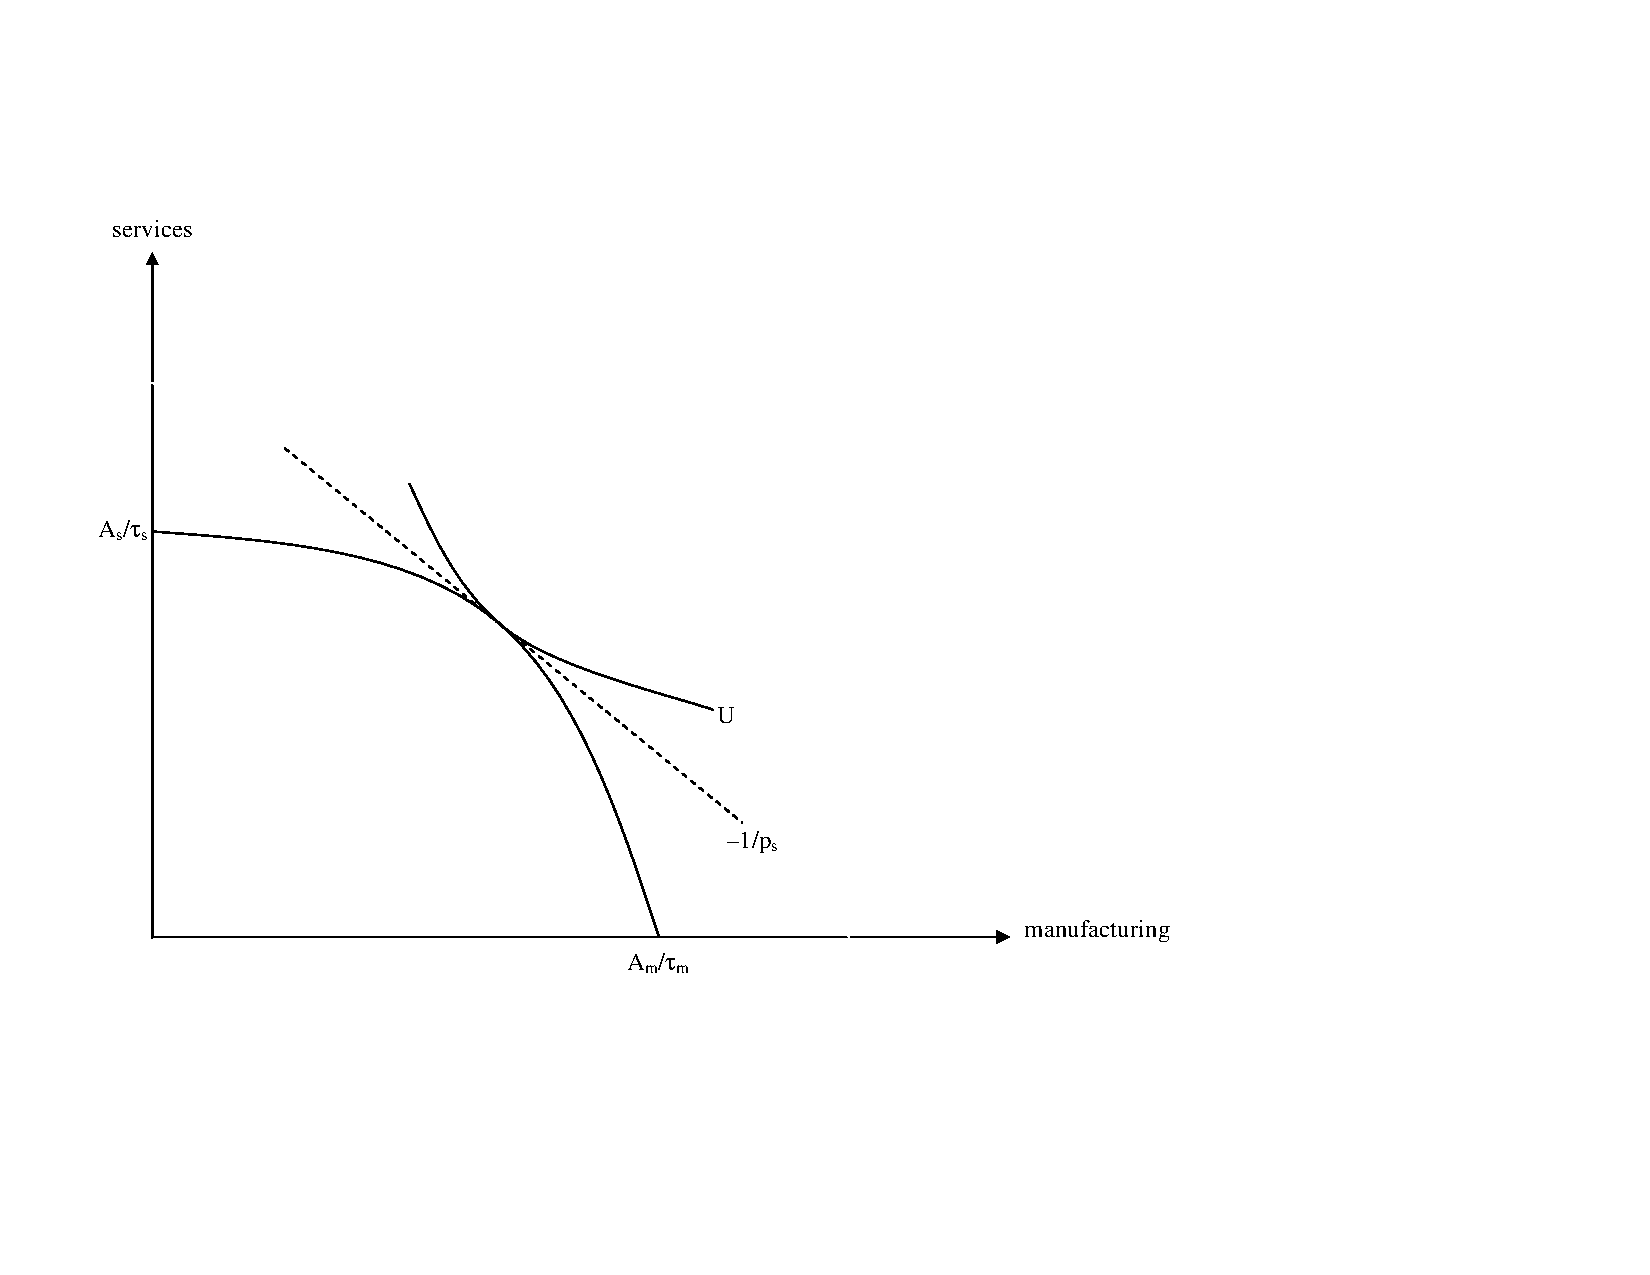
\includegraphics[width=\linewidth]{\directory/PPF-location-nonhomothetic-1.pdf}
    \end{center}}{
    \begin{center}
    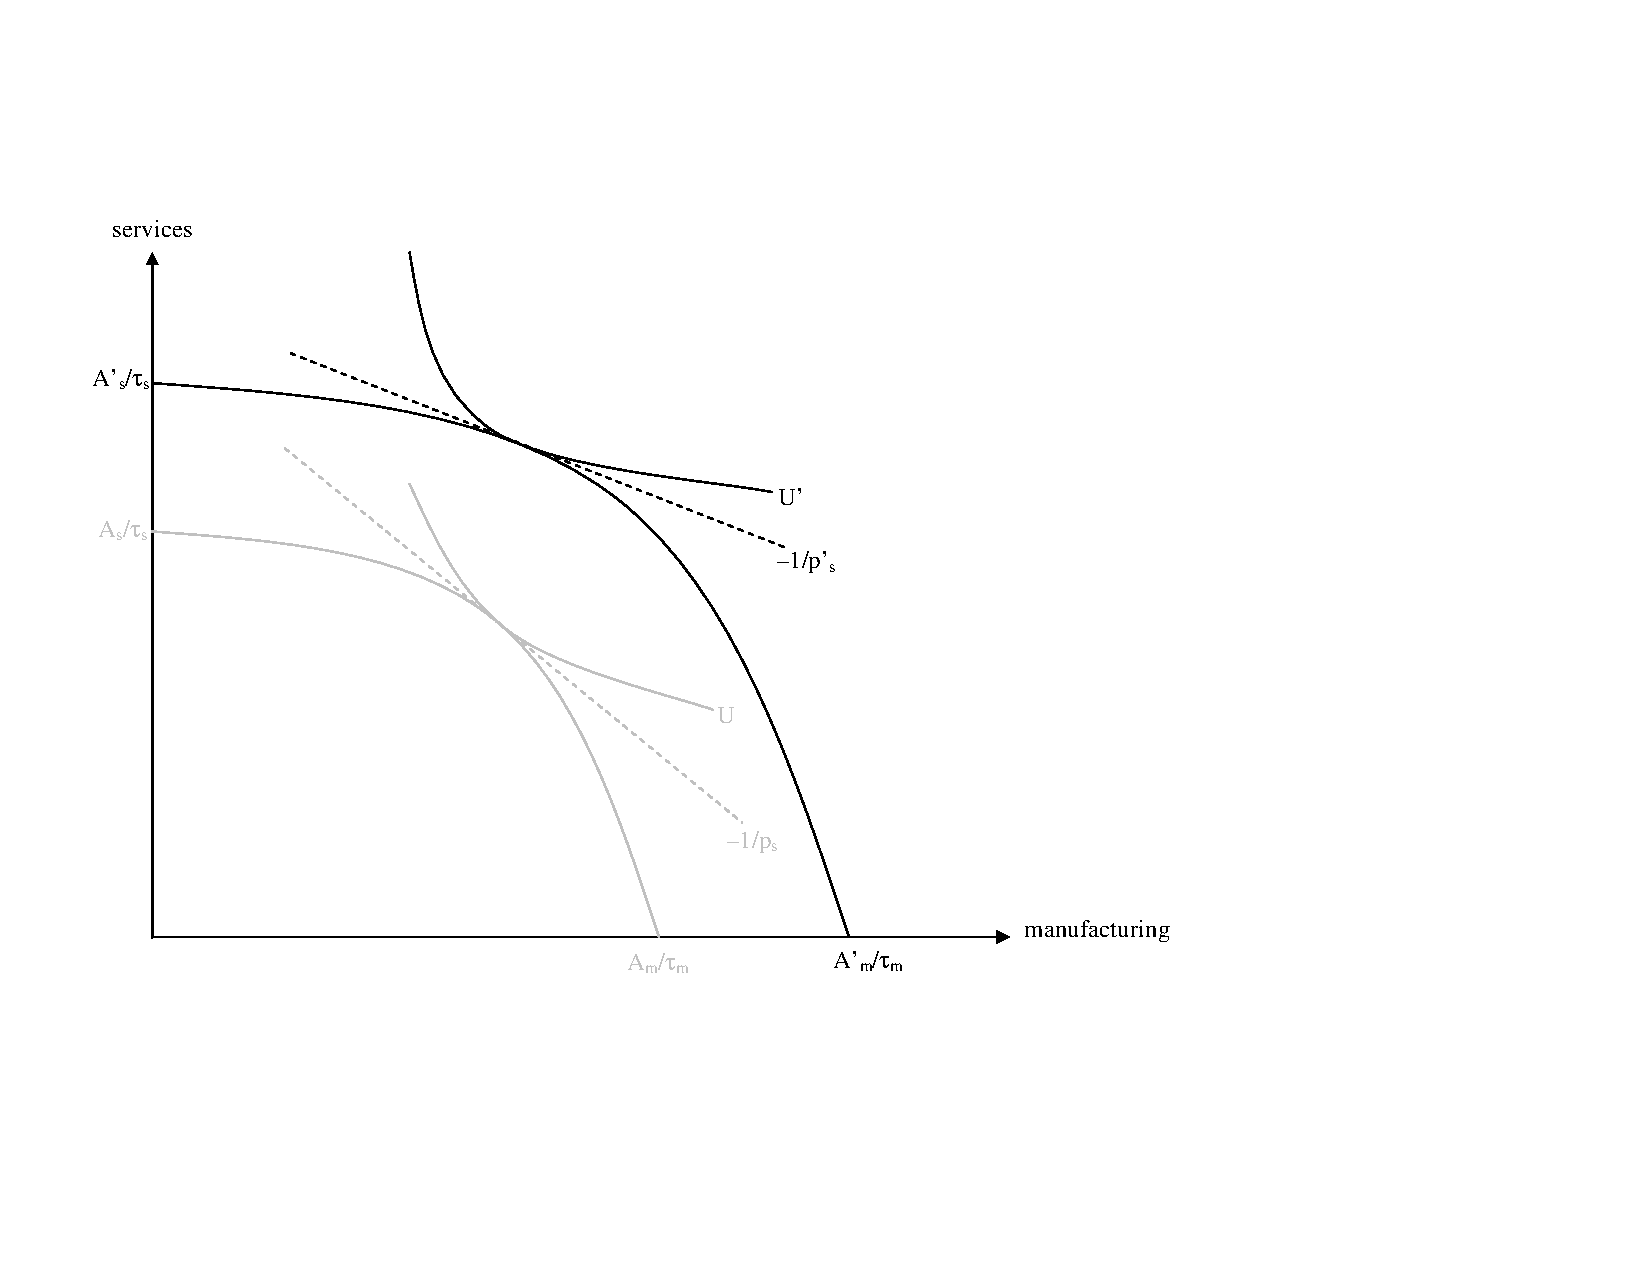
\includegraphics[width=\linewidth]{\directory/PPF-location-nonhomothetic-2.pdf}
    \end{center}}{
    \begin{center}
    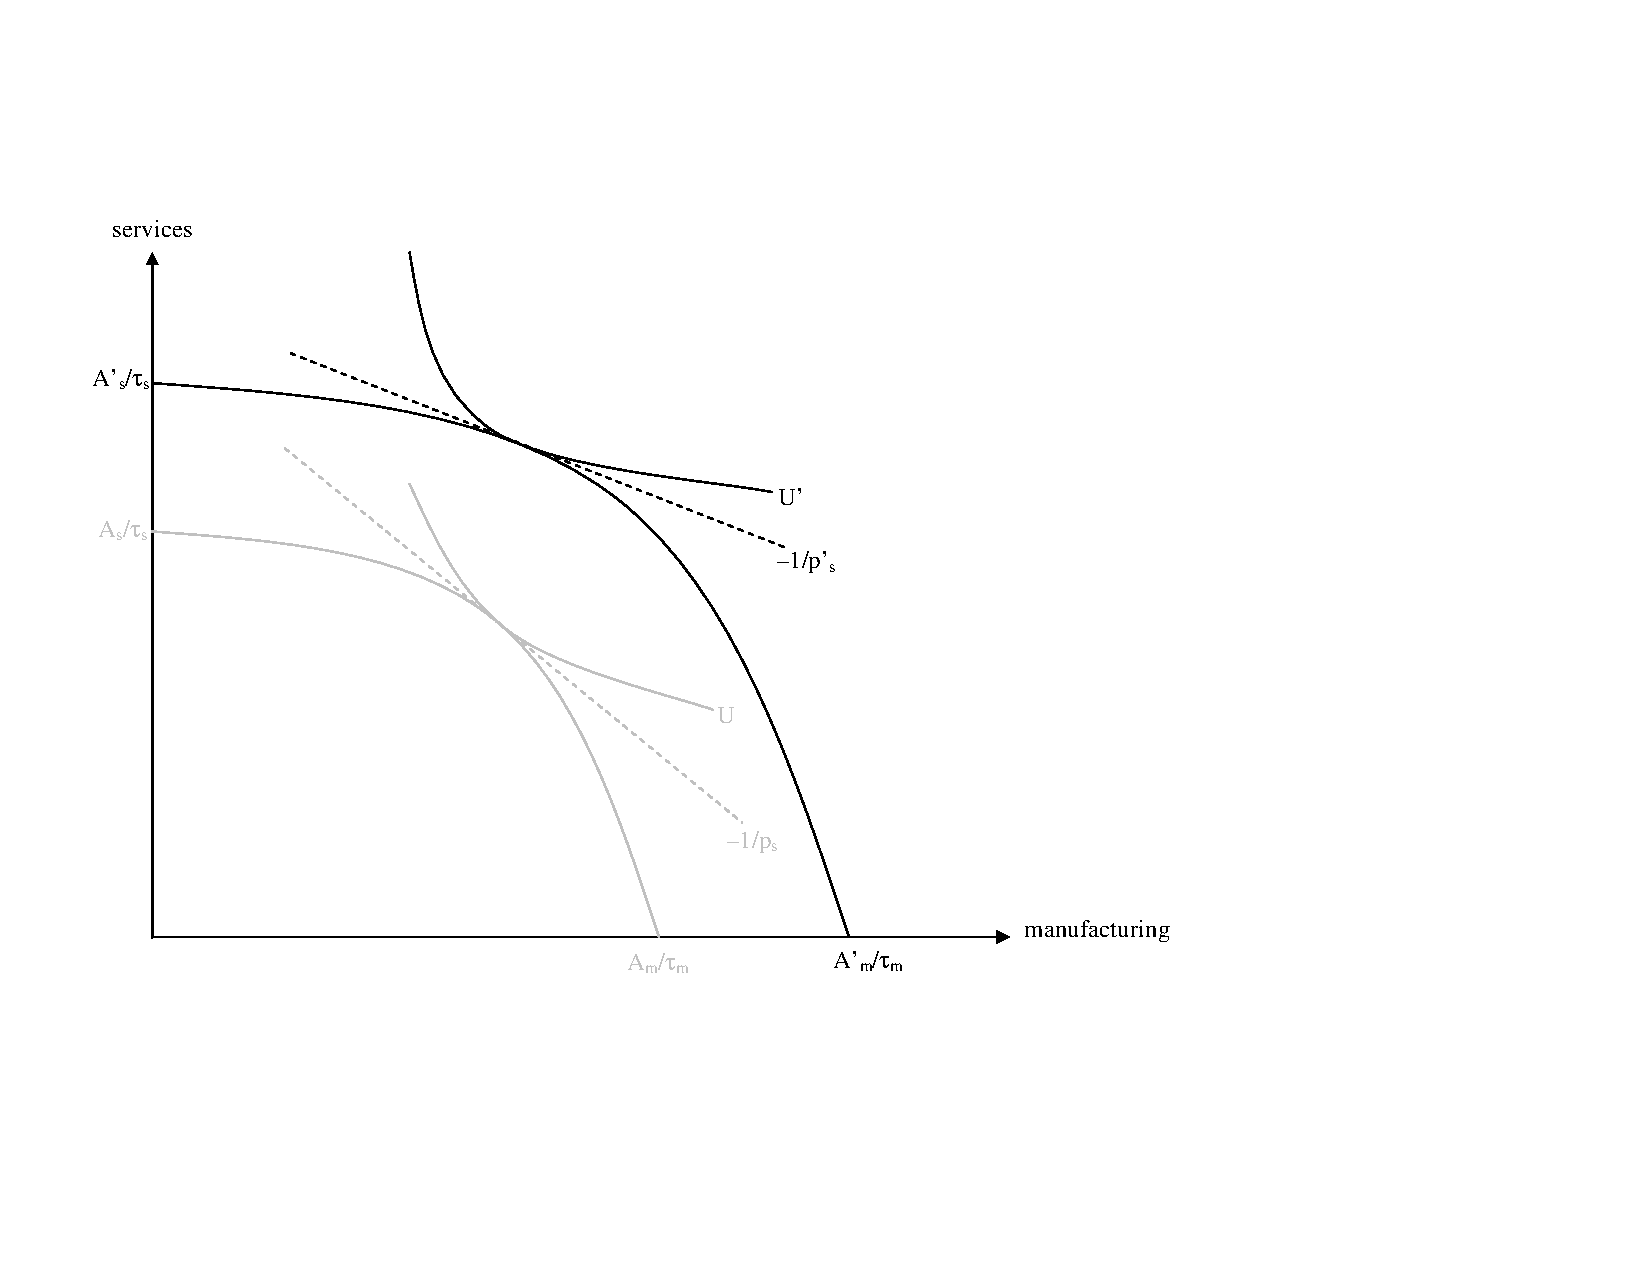
\includegraphics[width=\linewidth]{\directory/PPF-location-nonhomothetic-2.pdf}
    \end{center}}
\end{frame}

\begin{frame} \frametitle{Change in relative transport costs}
\hyperlink{development}{\beamerreturnbutton{return}}
\label{transport}
\temporal<2>{
    \begin{center}
    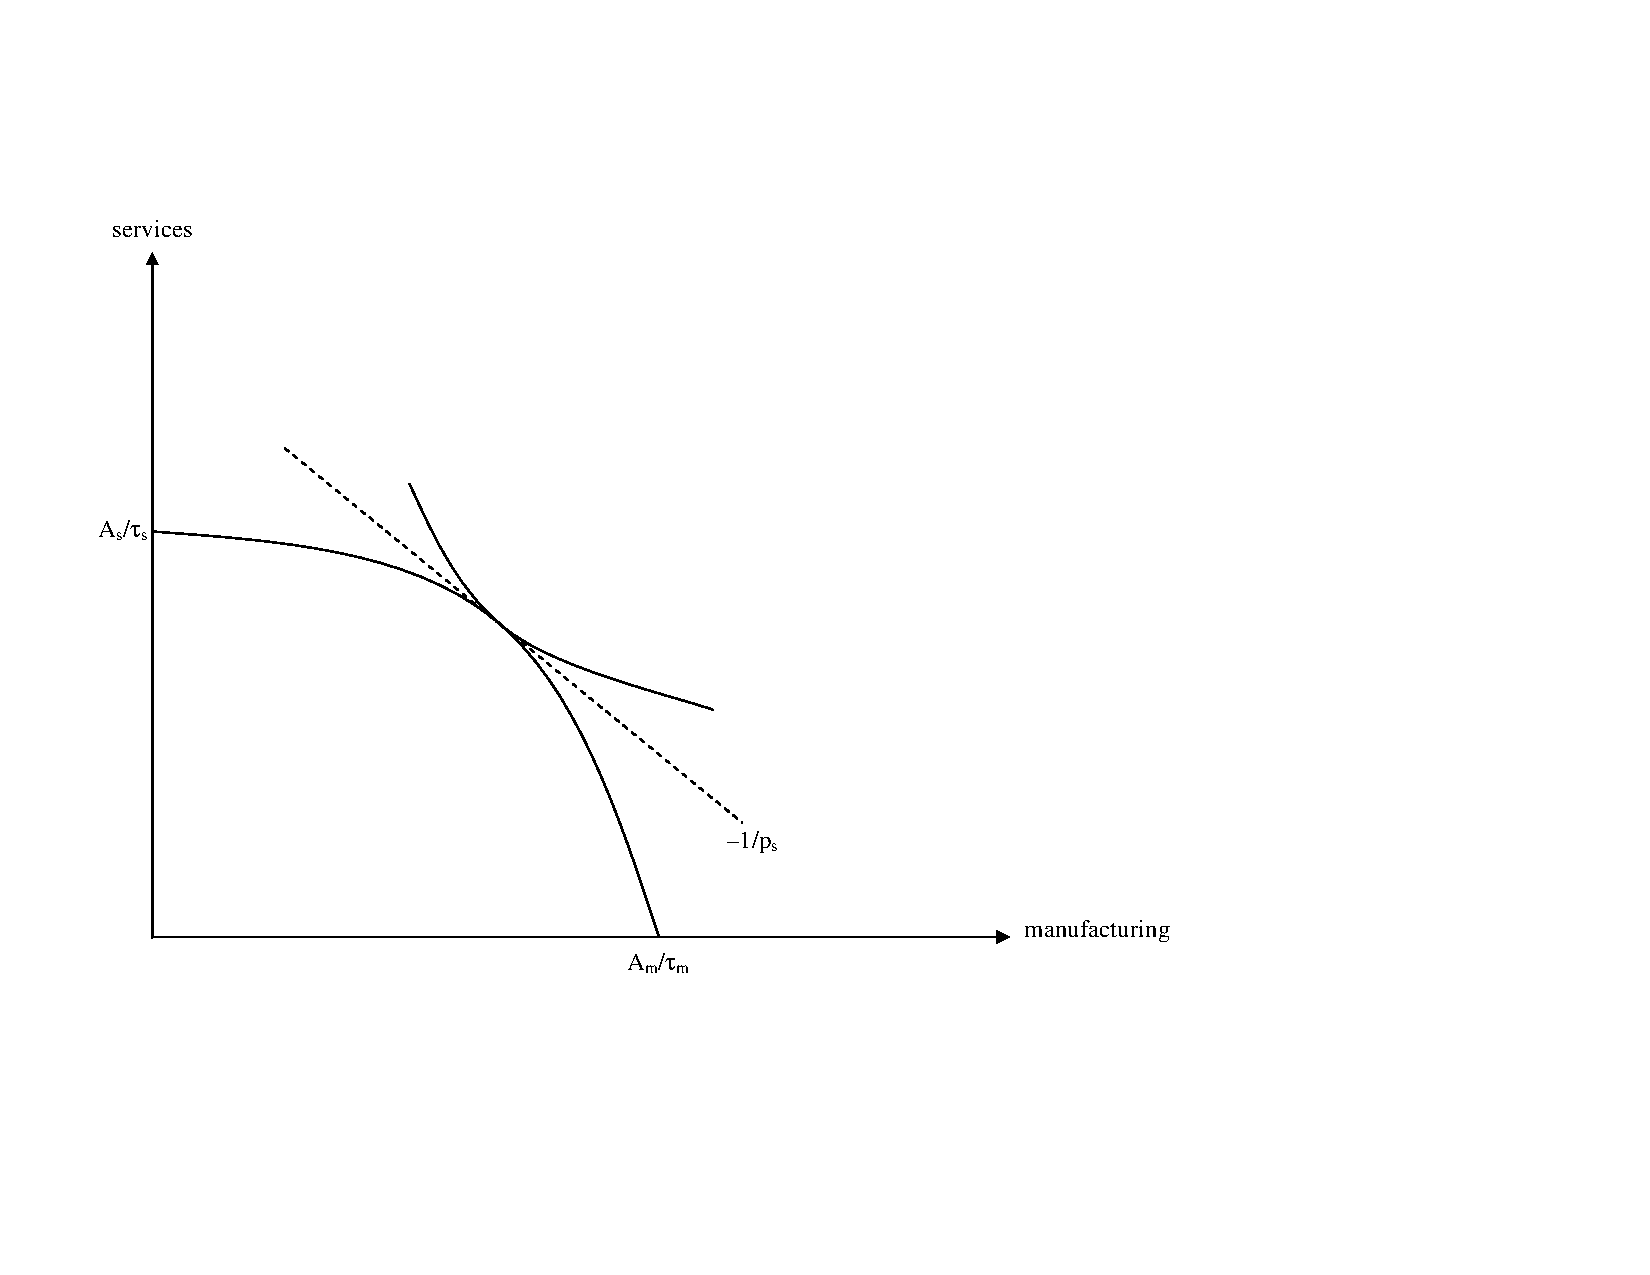
\includegraphics[width=\linewidth]{\directory/PPF-location-transport-1.pdf}
    \end{center}}{
    \begin{center}
    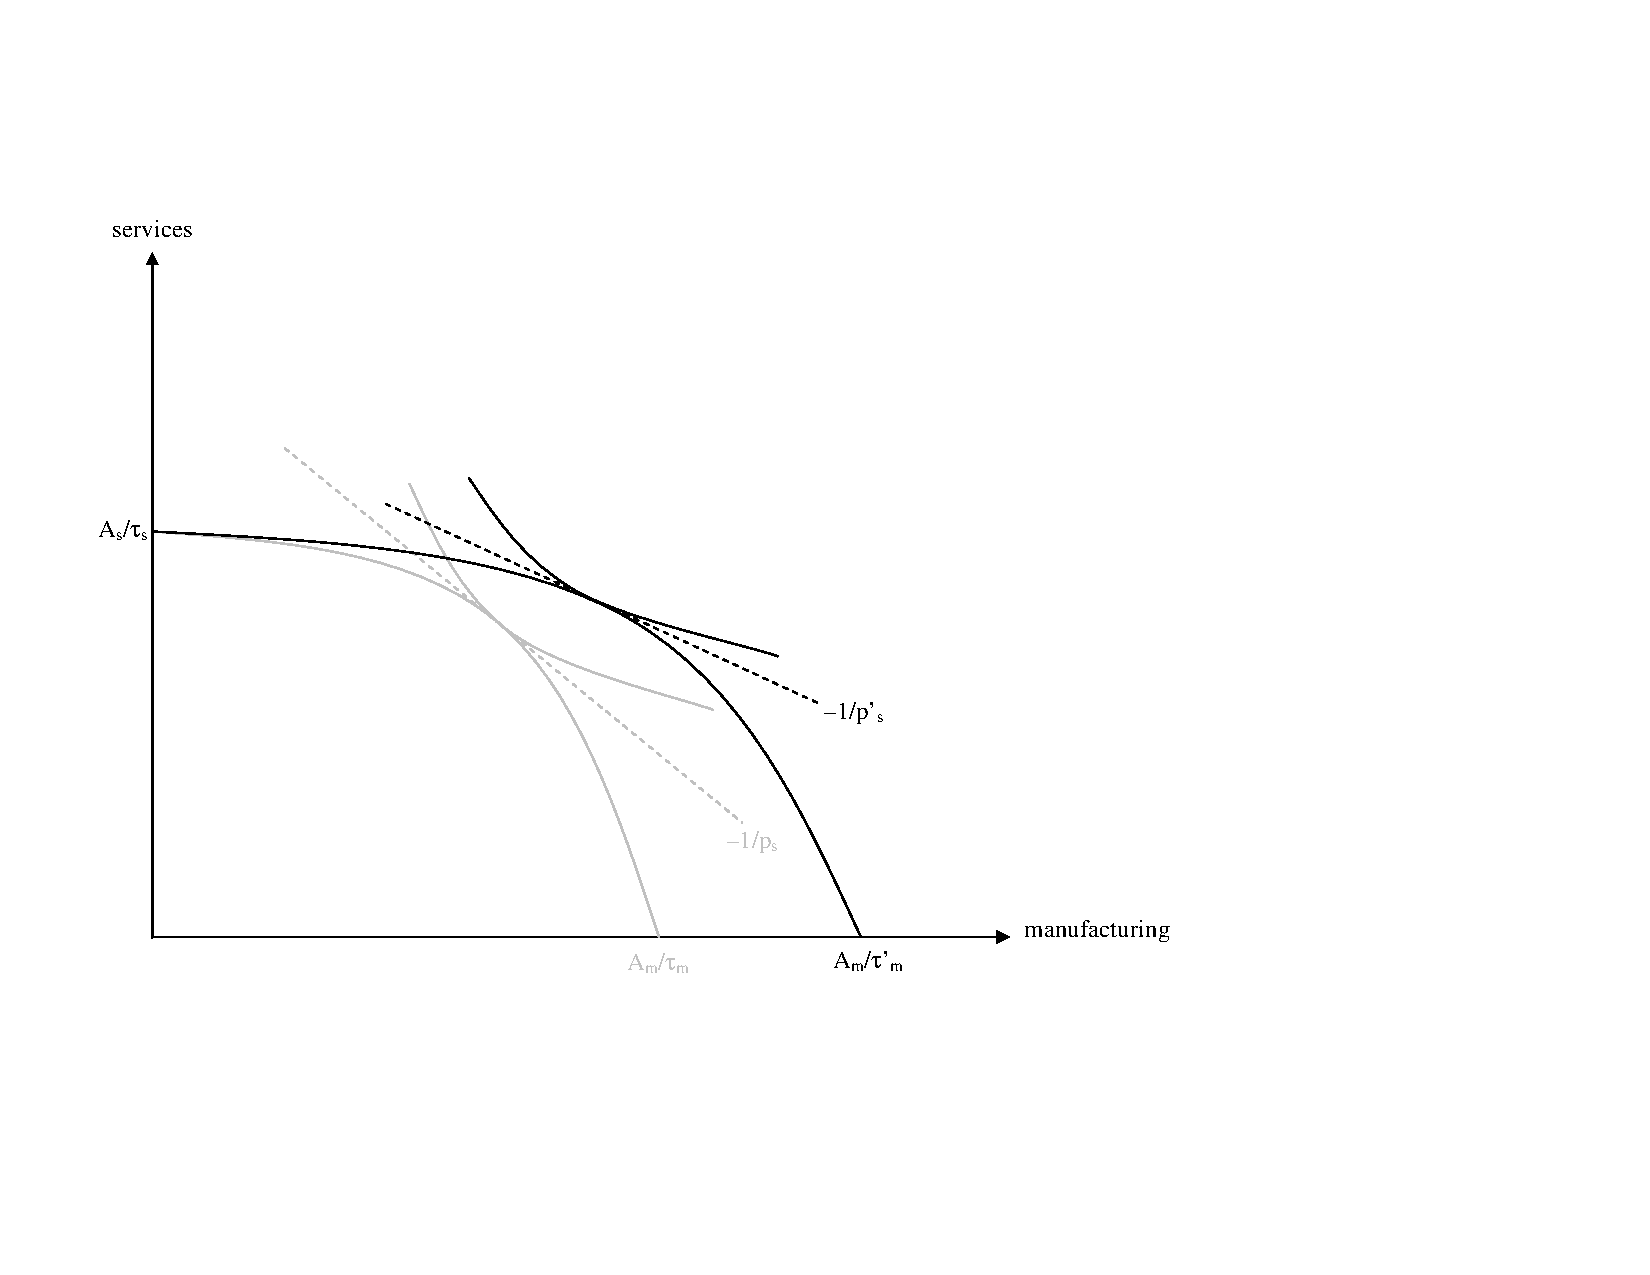
\includegraphics[width=\linewidth]{\directory/PPF-location-transport-2.pdf}
    \end{center}}{
    \begin{center}
    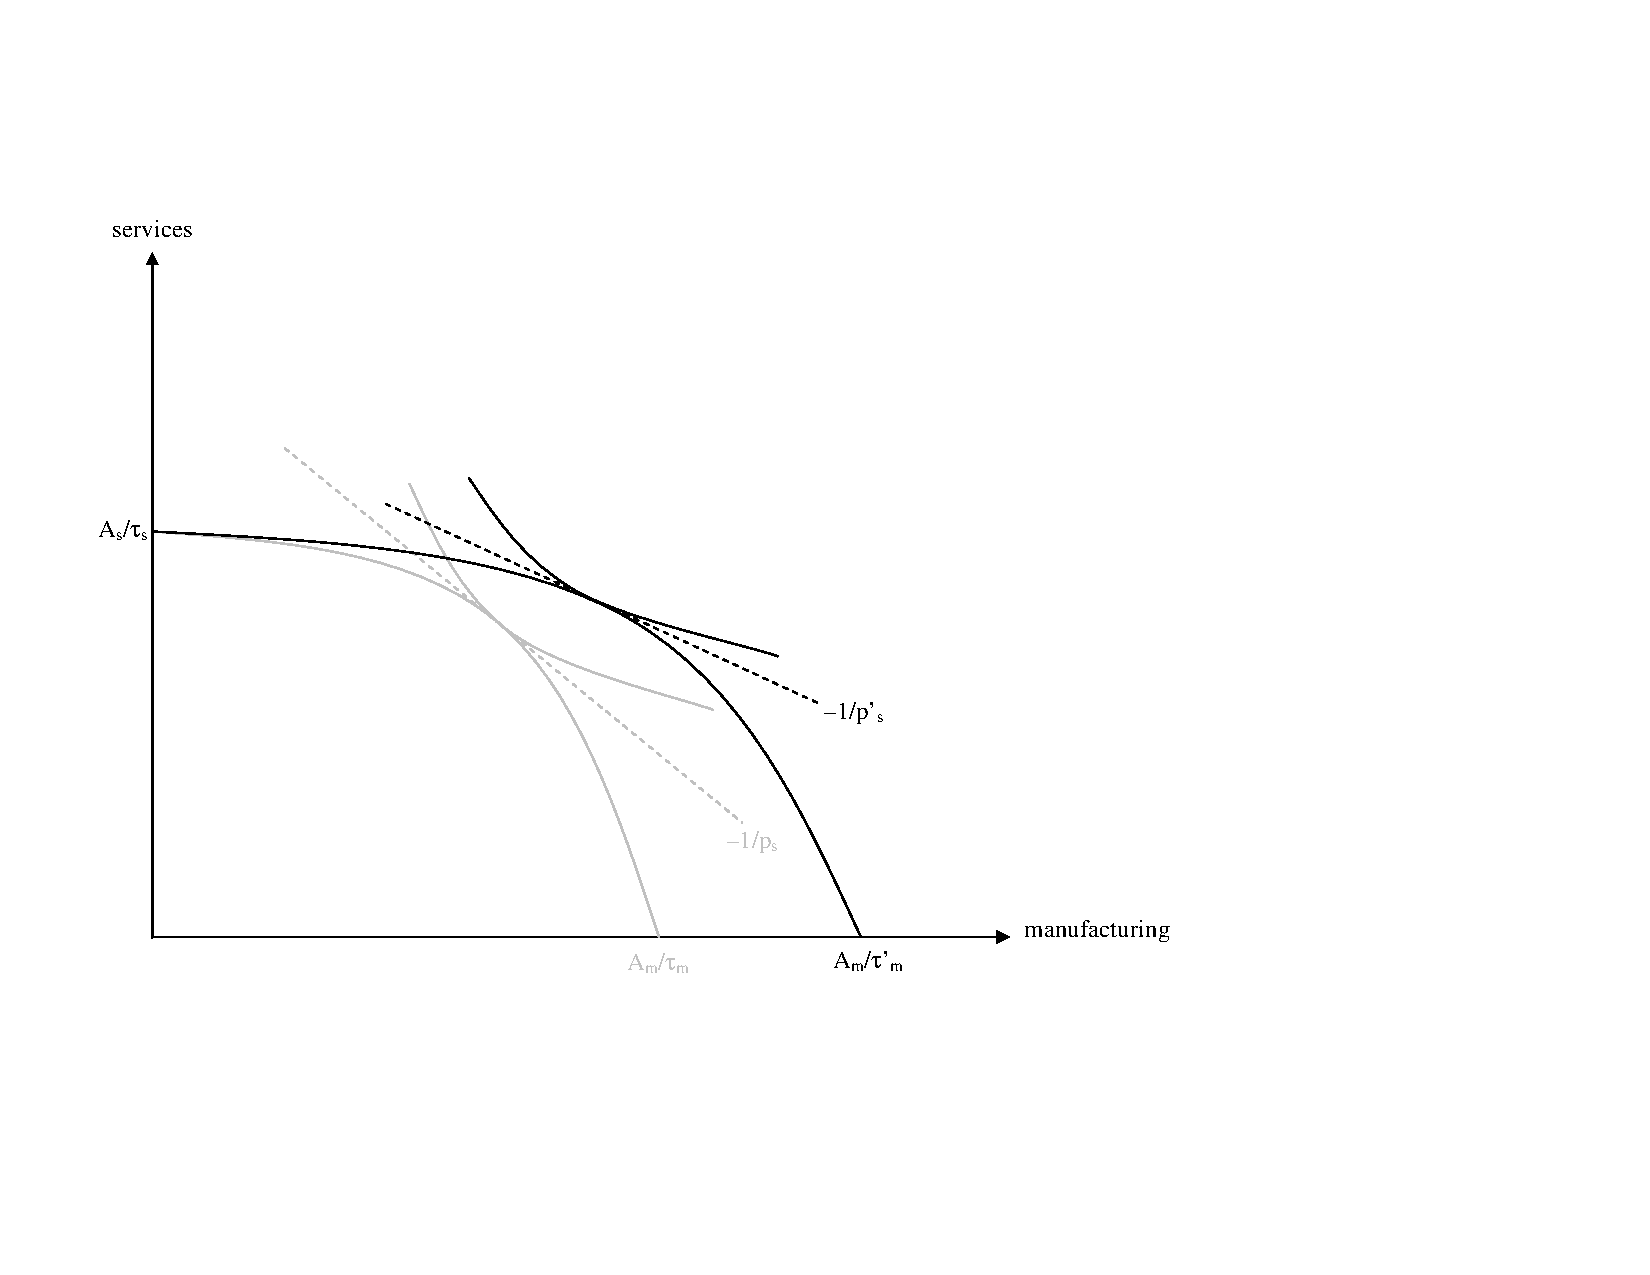
\includegraphics[width=\linewidth]{\directory/PPF-location-transport-2.pdf}
    \end{center}}
\end{frame}

\begin{frame} \frametitle{Housing} \hyperlink{development}{\beamerreturnbutton{return}}
\label{housing}
\temporal<2>{
    \begin{center}
    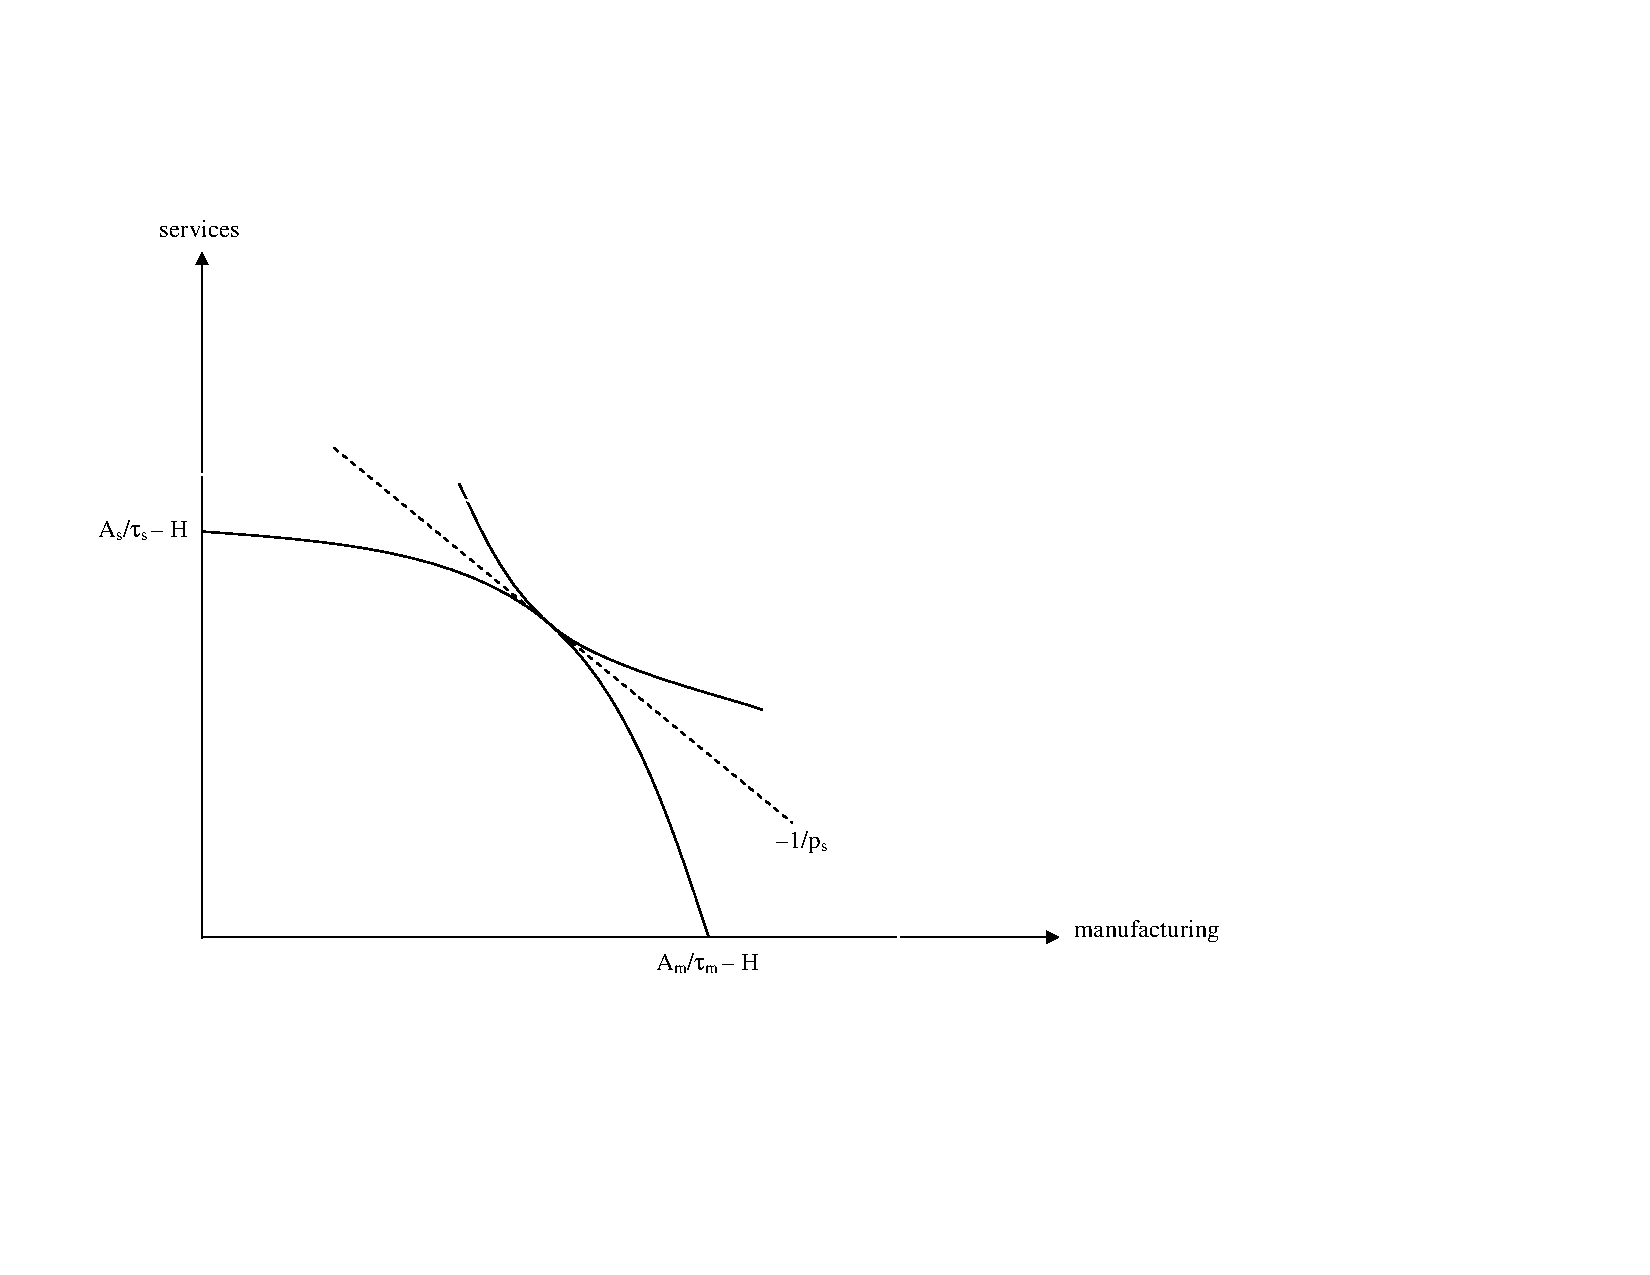
\includegraphics[width=\linewidth]{\directory/PPF-location-housing-1.pdf}
    \end{center}}{
    \begin{center}
    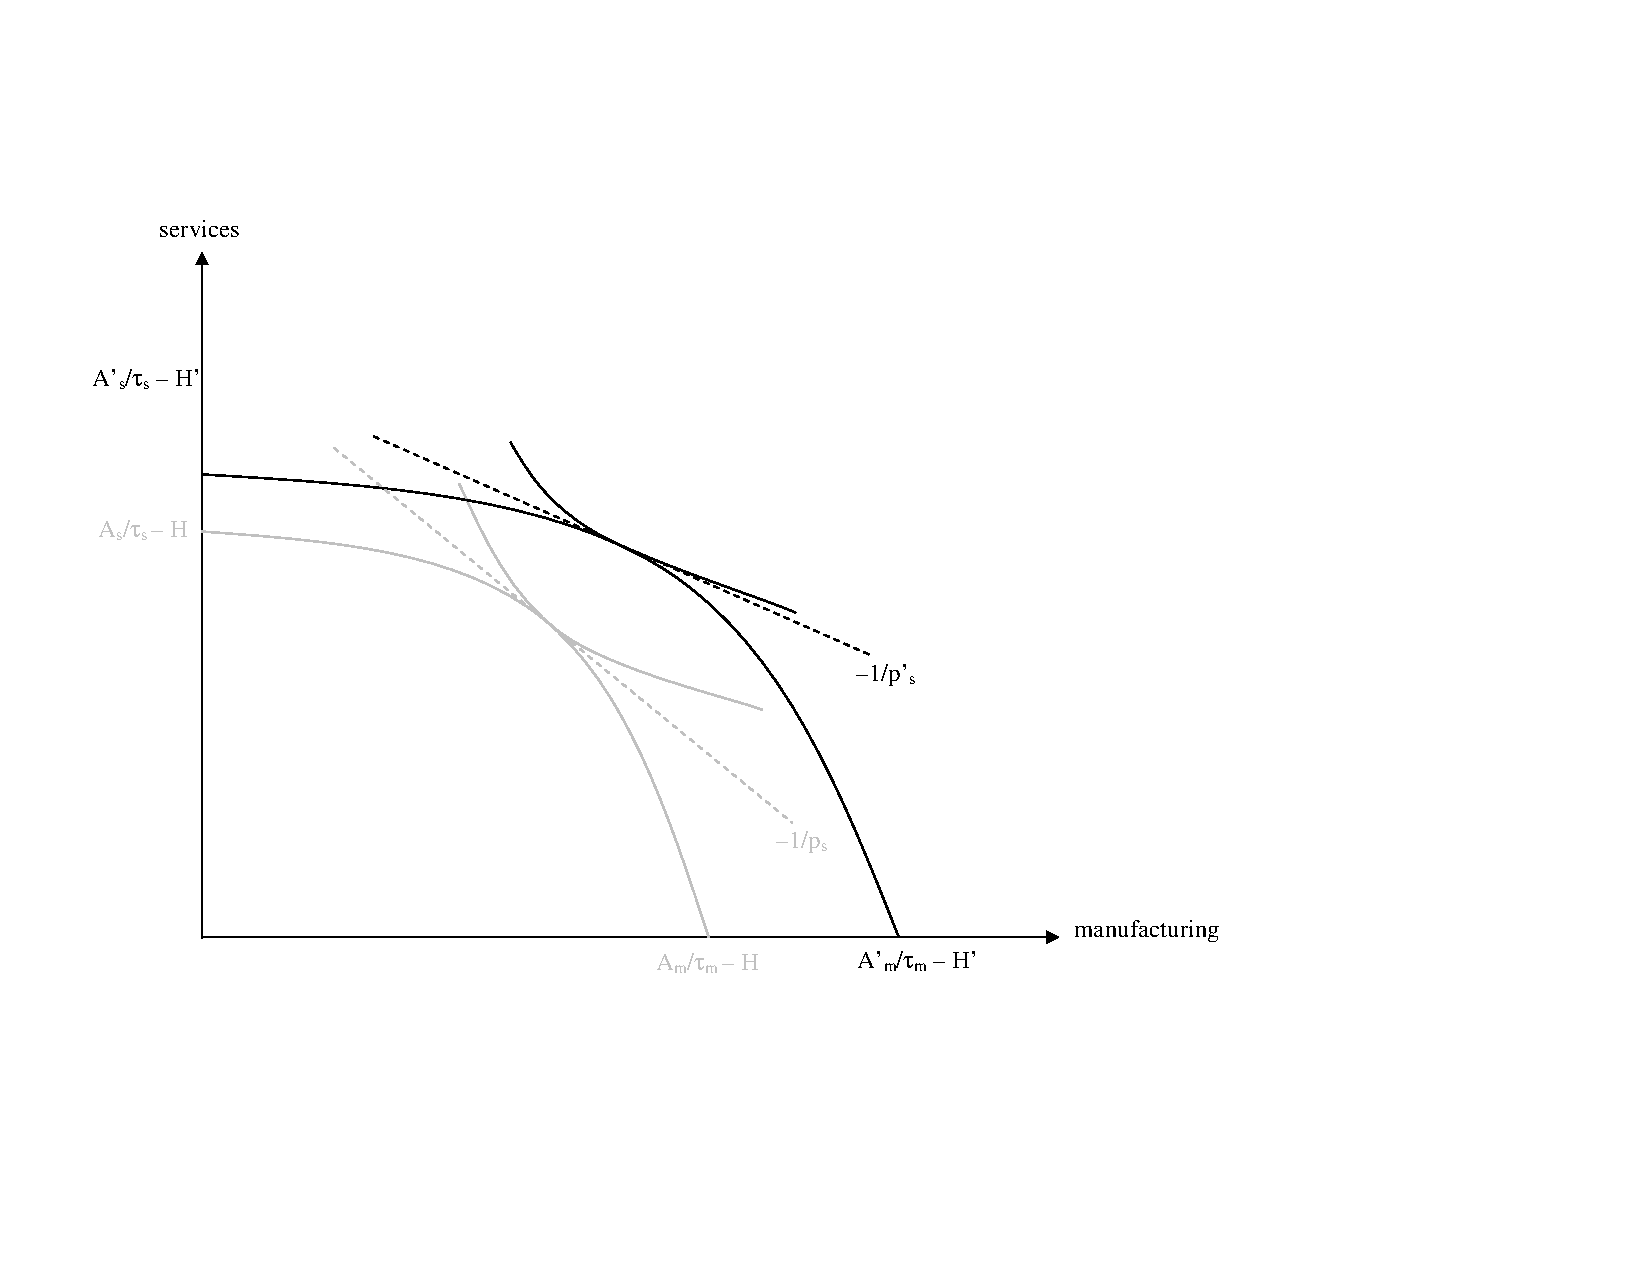
\includegraphics[width=\linewidth]{\directory/PPF-location-housing-2.pdf}
    \end{center}}{
    \begin{center}
    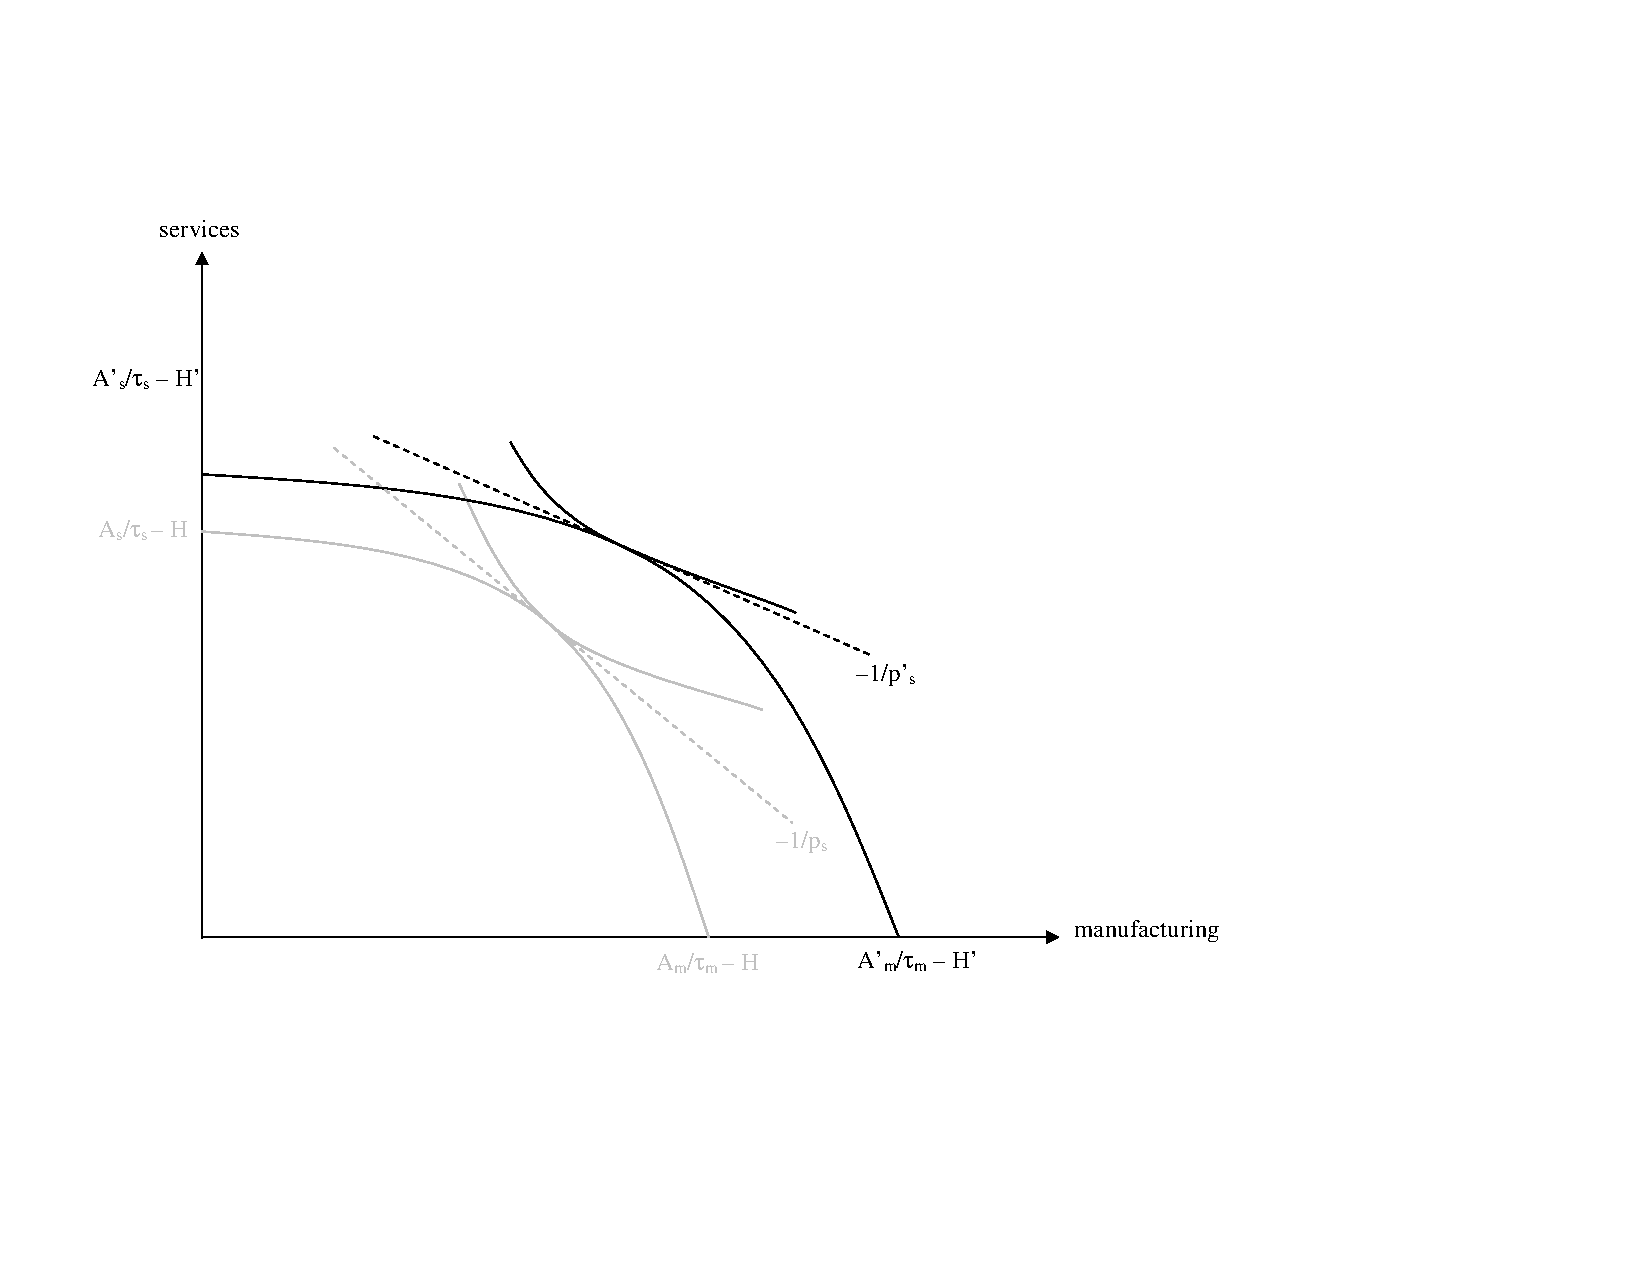
\includegraphics[width=\linewidth]{\directory/PPF-location-housing-2.pdf}
    \end{center}}
\end{frame}



%% explain flat line first. then explain why the other line is curved. this starts to look like the bhagwati story. will need something that makes rural land abundant relative to urban land

%% graph of PPF. analogy to bhagwati story


\end{document}



%% insert some formal MRT slides here
\begin{frame}\frametitle{Technology based explanations I.}

\begin{block}{Technology}
Product $i$ is produced using $A_iF_i(k_i,n_i)$.
\end{block}

\begin{block}{Production possibilities set}
Feasible $(m,s)$ such that $k_m+k_s = K$ and $n_m+n_s = N$.
\end{block}

\begin{block}{Marginal rate of transformation}
Number of $m$s sacrificed for a unit of $s$:
\[
MRT=\frac{A_mF_{mk}(k_m,n_m)}{A_sF_{sk}(k_s,n_s)}
\]
\end{block}

\begin{block}{Relative price}
In equilibrium, the relative price is pinned down by the MRT.
\end{block}

\end{frame}






\begin{frame}\frametitle{Predictions}


As productivity increases,
\begin{enumerate}
    \item residential land increases,
    \item home prices increase,
    \item the rent gradient becomes steeper,
    \item tradable industries move away from center,
    \item services become more expensive,
    \item labor productivity increases faster in manufacturing.
%   \item employment becomes more concentrated.
\end{enumerate}
\begin{enumerate}
    \item[7.] All of these effects are stronger for more densely populated countries.
\end{enumerate}
\end{frame}
\time 2
